\documentclass{article}
\usepackage{graphicx} % Required for inserting images
\usepackage{hyperref}
\usepackage{amsmath}
\usepackage{longtable}
\usepackage{booktabs}

%\usepackage{biblatex}
\usepackage[backend=biber,
style=authoryear,
citestyle=authoryear]{biblatex} 
\addbibresource{latex/bibliograph.bib}

\title{Prospectus Proposal}
\author{Joseph Fish}
\date{March 2024}


\begin{document}

\section{Motivation}

The vast majority of low income renters in America rent from the private market. These rental markets are characterized by surprisingly high prices and supernormal profits \parencite{Desmond_2019, Damen_2025,Eisfeldt_2015}, low maintenance, minimal entry, high search frictions, and high rates of tenant default \parencite{humphries-2024} and eviction \parencite{Gromis-et-al-2022}. The welfare costs to tenants through eviction are substantive \parencite{collison-et-al-2023, graetz-at-al-2023} and are compounded by likely monopoly rents in low income housing as well as documented predatory behavior by some low income landlords \parencite{desmond-evicted}. Because of these negative effects on tenants there is obvious scope and justification for regulation of and intervention into the low income rental market. Additionally, because most cities are relatively cash constrained, first best policies such as transfers are generally infeasible.\\

Despite the aforementioned market failures, because the private market provides the majority of housing to low income renters, regulation has to be careful not to induce widespread exit of low income landlords as this has been linked to increased rent prices \parencite{collinson2024eviction}, declining housing supply \parencite{diamond-2019}, and homelessness \parencite{pinto2024sro}. As such, optimal regulation of the low income rental market is ex-ante unclear and relies on understanding the scope of market power in these markets as well as the exit thresholds for low-income landlords.\\   

This prospectus makes two contributions to the literature on low income housing and, more broadly, to how we should think about market power and landlord decisions in the rental market. In my job market paper

% Evictions in America are both remarkably common and remarkably concentrated. Each year, there are around 3.6 million eviction filings. These filings disproportionately occur within certain cities, within certain neighborhoods in those cities, and within certain buildings inside those neighborhoods. In the most extreme cases, like in Tuscon, Arizona, 300 buildings are responsible for over 66\% of eviction filings. In Philadelphia, only around 15\% of rental units will file an eviction in a given year, and about 10\% of all eviction filings come from just 2\% of units, and 25\% come from 10\% of all rental units. \\

% Going further, serial evictions, which are consecutive (serial) filings on the same tenant at the same address, are also concentrated within particular sets of landlords. These filings are typically thought to be ways in which landlords use the court system as debt collectors as they do not result in a change in tenancy, even thought the landlord typically wins a writ of possession. Additionally, statements from the National  Apartment Association (NAA) highlight they think their ability to evict tenants is an important part of why they remain in the low income rental market. Taken together, there is substantial evidence that eviction is an important component of a particular kind of landlord's business model. \\


\section{Empirical Setting}

The empirical setting for this project will be Philadelphia, Pennsylvania. Philadelphia is an ideal city for a number of reasons. On the demographic side, Philadelphia is the largest poor city in America, with a high eviction rate, high segregation, and a large Black population, making it a very useful case study for understanding America's low income housing market. On the data side, Philadelphia is unique in that it has a rental registry, meaning I can see exactly which properties are rental units in each year. Other studies have had to rely on owner occupancy exemptions to identify rental properties, which is problematic because it conflates rental units with Airbnbs and vacation homes. \\

Additionally, Philadelphia has very good historical eviction data, and, importantly, the eviction data contain contract rents, which let me see normally hard to observe rent prices for low income units. Finally, on the policy side, Philadelphia had a large change in their tenant protections in 2022, where they now make eviction cases go through mediation, leading to an approximately 30\% decline in eviction filings, relative to a pre-pandemic baseline.

\section{Stylized Facts about Philadelphia's Low Income Housing Market}

In this section, I lay out a series of motivating empirical facts about Philadelphia's low income housing market. Beginning with a map of Philadelphia (figure \ref{fig:philly-map}), I show that evictions in Philadelphia are geographically very concentrated in the predominately poor and highly segregated neighborhoods of West and North Philadelphia.


\begin{figure}[htbp]
    \centering
    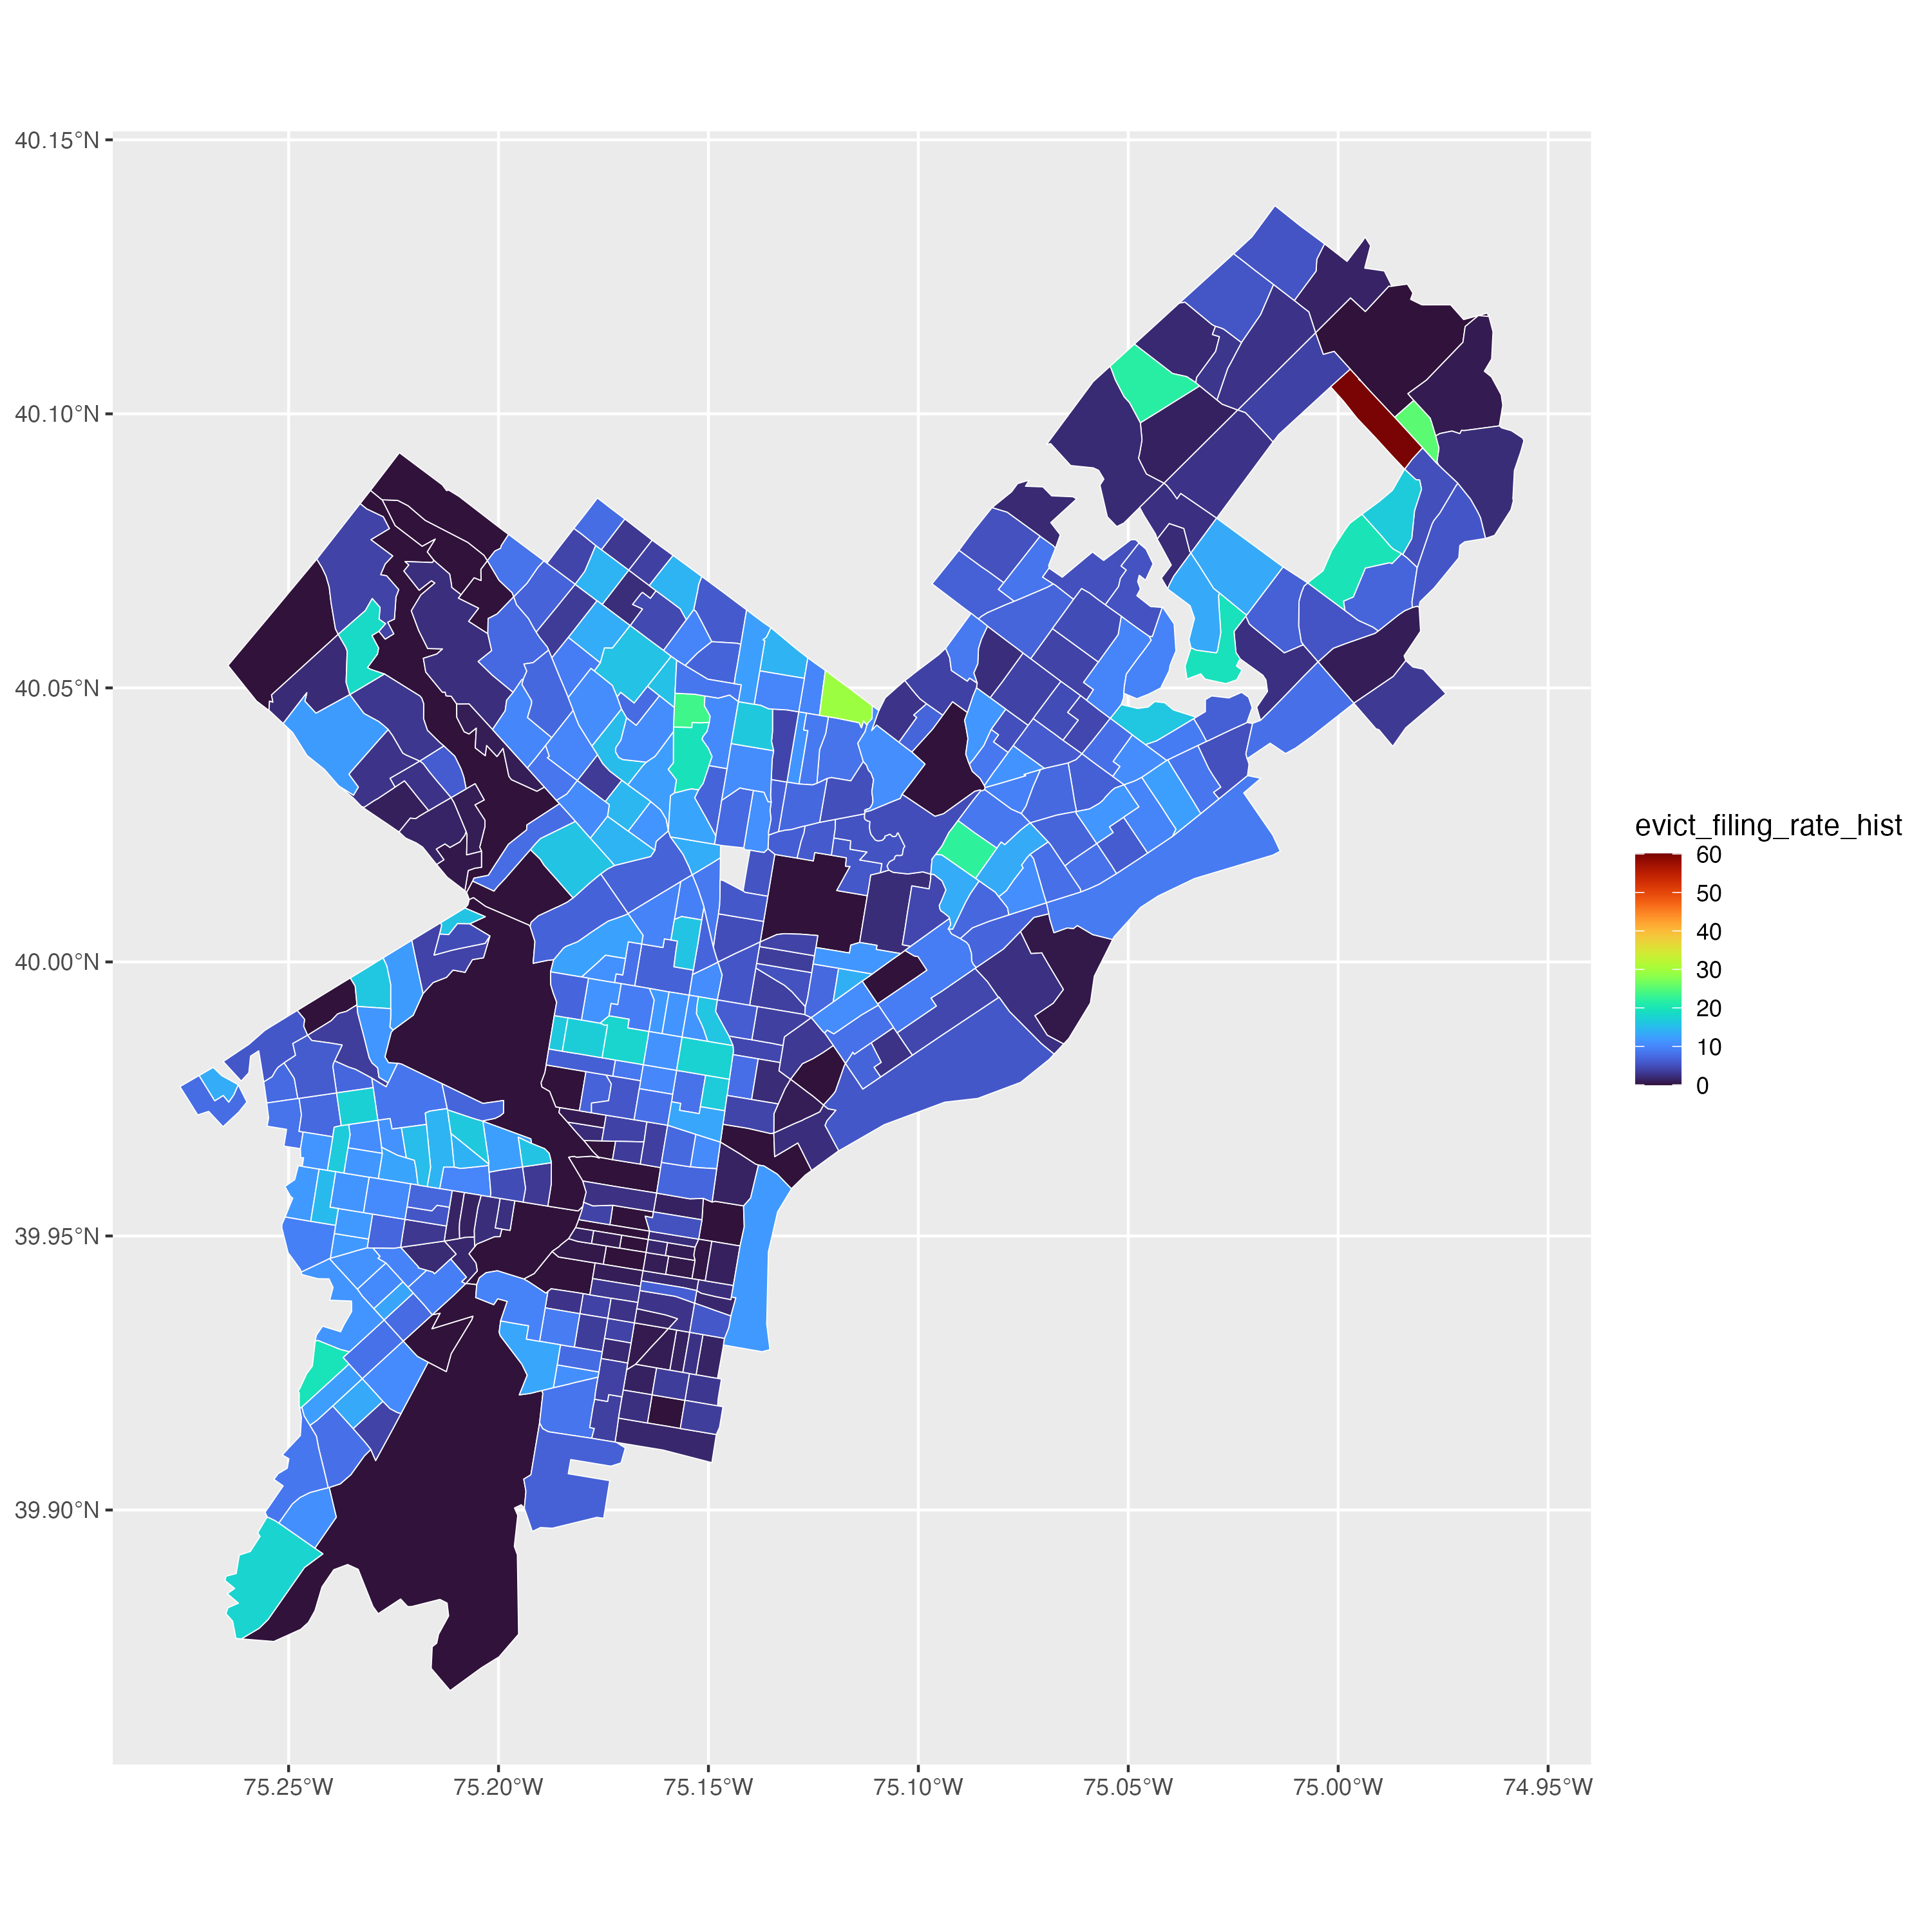
\includegraphics[width=1\linewidth]{figs/evict_filing_rate_hist.png}
    \caption{Evictions in Philadelphia (2019)}
    \label{fig:philly-map}
\end{figure}

Secondly, I show that, when looking across properties, evictions are concentrated in a handful of buildings. To show this, I merged the eviction data, which contain the defendant's address, with the rental registry and the parcel data in Philadelphia. This lets me know which properties are rental units in a given year, as well as the number of rental units that are in each property. Doing this allows me to plot the CDF of eviction filings alongside the CDF of rental units. \\

As figure \ref{fig:philly-evict-parcel} shows, the vast majority of rental units do not file an eviction in a typical year. Of the properties that do file an eviction, most file only one. Collectively, about 10\% of all eviction filings come from just 2\% of units. \\

\begin{figure}[htbp]
    \centering
    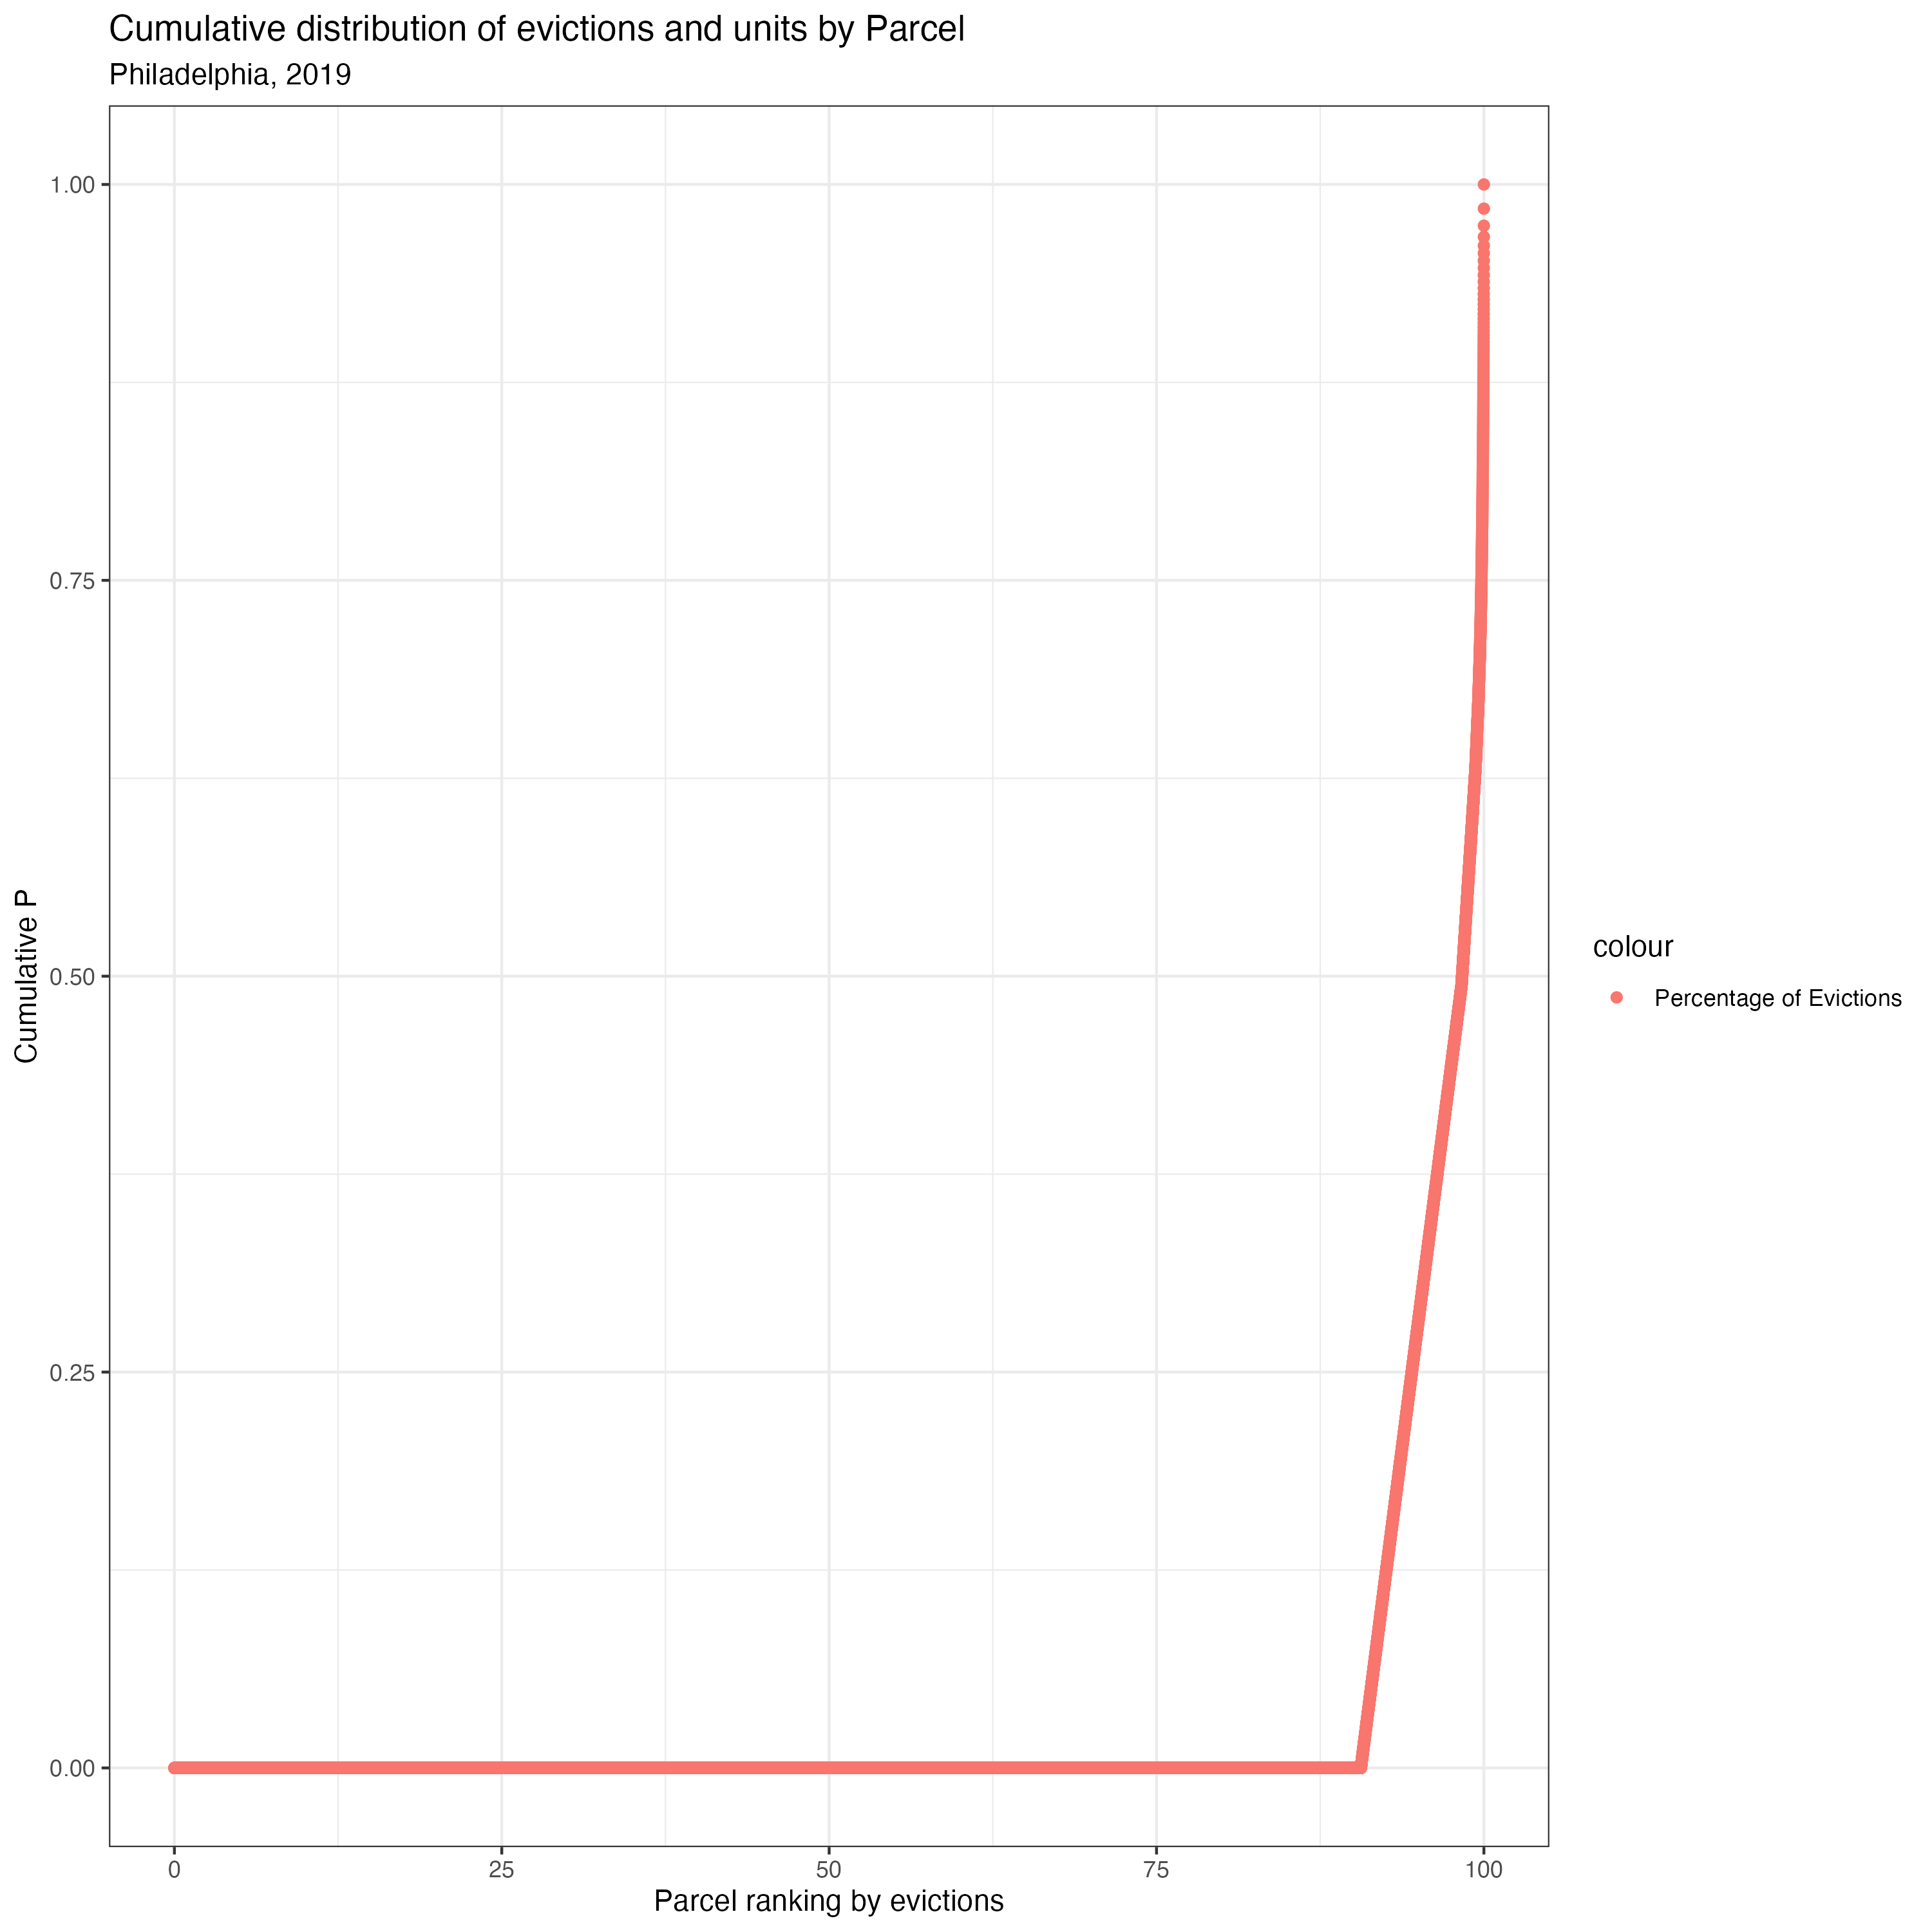
\includegraphics[width=1\linewidth]{figs/cumulative_evict_dist_parcels.png}
    \caption{Evictions in Philadelphia}
    \label{fig:philly-evict-parcel}
\end{figure}

Third, in table \ref{tab:philly-rent},I group eviction filings by whether they were filed by one of the top-100 evicting plaintiffs in each year. I show that there are not substantial differences in rent prices between filings by high / low evicting plaintiffs.\\

\begin{table}[htbp]
    \begin{longtable}{l|rrrr}
\caption*{
{\large Summary Statistics on Philadelphia Rent Prices} \\ 
{\small 2010-2019}
} \\ 
\toprule
\multicolumn{1}{l}{} & \multicolumn{2}{c}{Rent} & \multicolumn{2}{c}{Number of Evictions} \\ 
\cmidrule(lr){2-3} \cmidrule(lr){4-5}
\multicolumn{1}{l}{} & non-Top Evictor & Top Evictor & non-Top Evictor & Top Evictor \\ 
\midrule\addlinespace[2.5pt]
2010 & $675$ & $634$ & 14649 & 6674 \\ 
2011 & $685$ & $654$ & 14979 & 6498 \\ 
2012 & $700$ & $654$ & 15271 & 6642 \\ 
2013 & $700$ & $675$ & 15366 & 6064 \\ 
2014 & $725$ & $707$ & 15645 & 6257 \\ 
2015 & $750$ & $725$ & 14395 & 5891 \\ 
2016 & $750$ & $800$ & 14994 & 5622 \\ 
2017 & $775$ & $825$ & 14627 & 5748 \\ 
2018 & $800$ & $970$ & 11987 & 3735 \\ 
2019 & $850$ & $1,050$ & 11763 & 3473 \\ 
\bottomrule
\end{longtable}


    \caption{Philadelphia Rent}
    \label{tab:philly-rent}
\end{table}


% Finally, in figure \ref{fig:philly-year}, I show that evictions declined substantially during COVID and have held at lower rates than the pre-pandemic baseline. \\

% \begin{figure}[htbp]
%     \centering
%     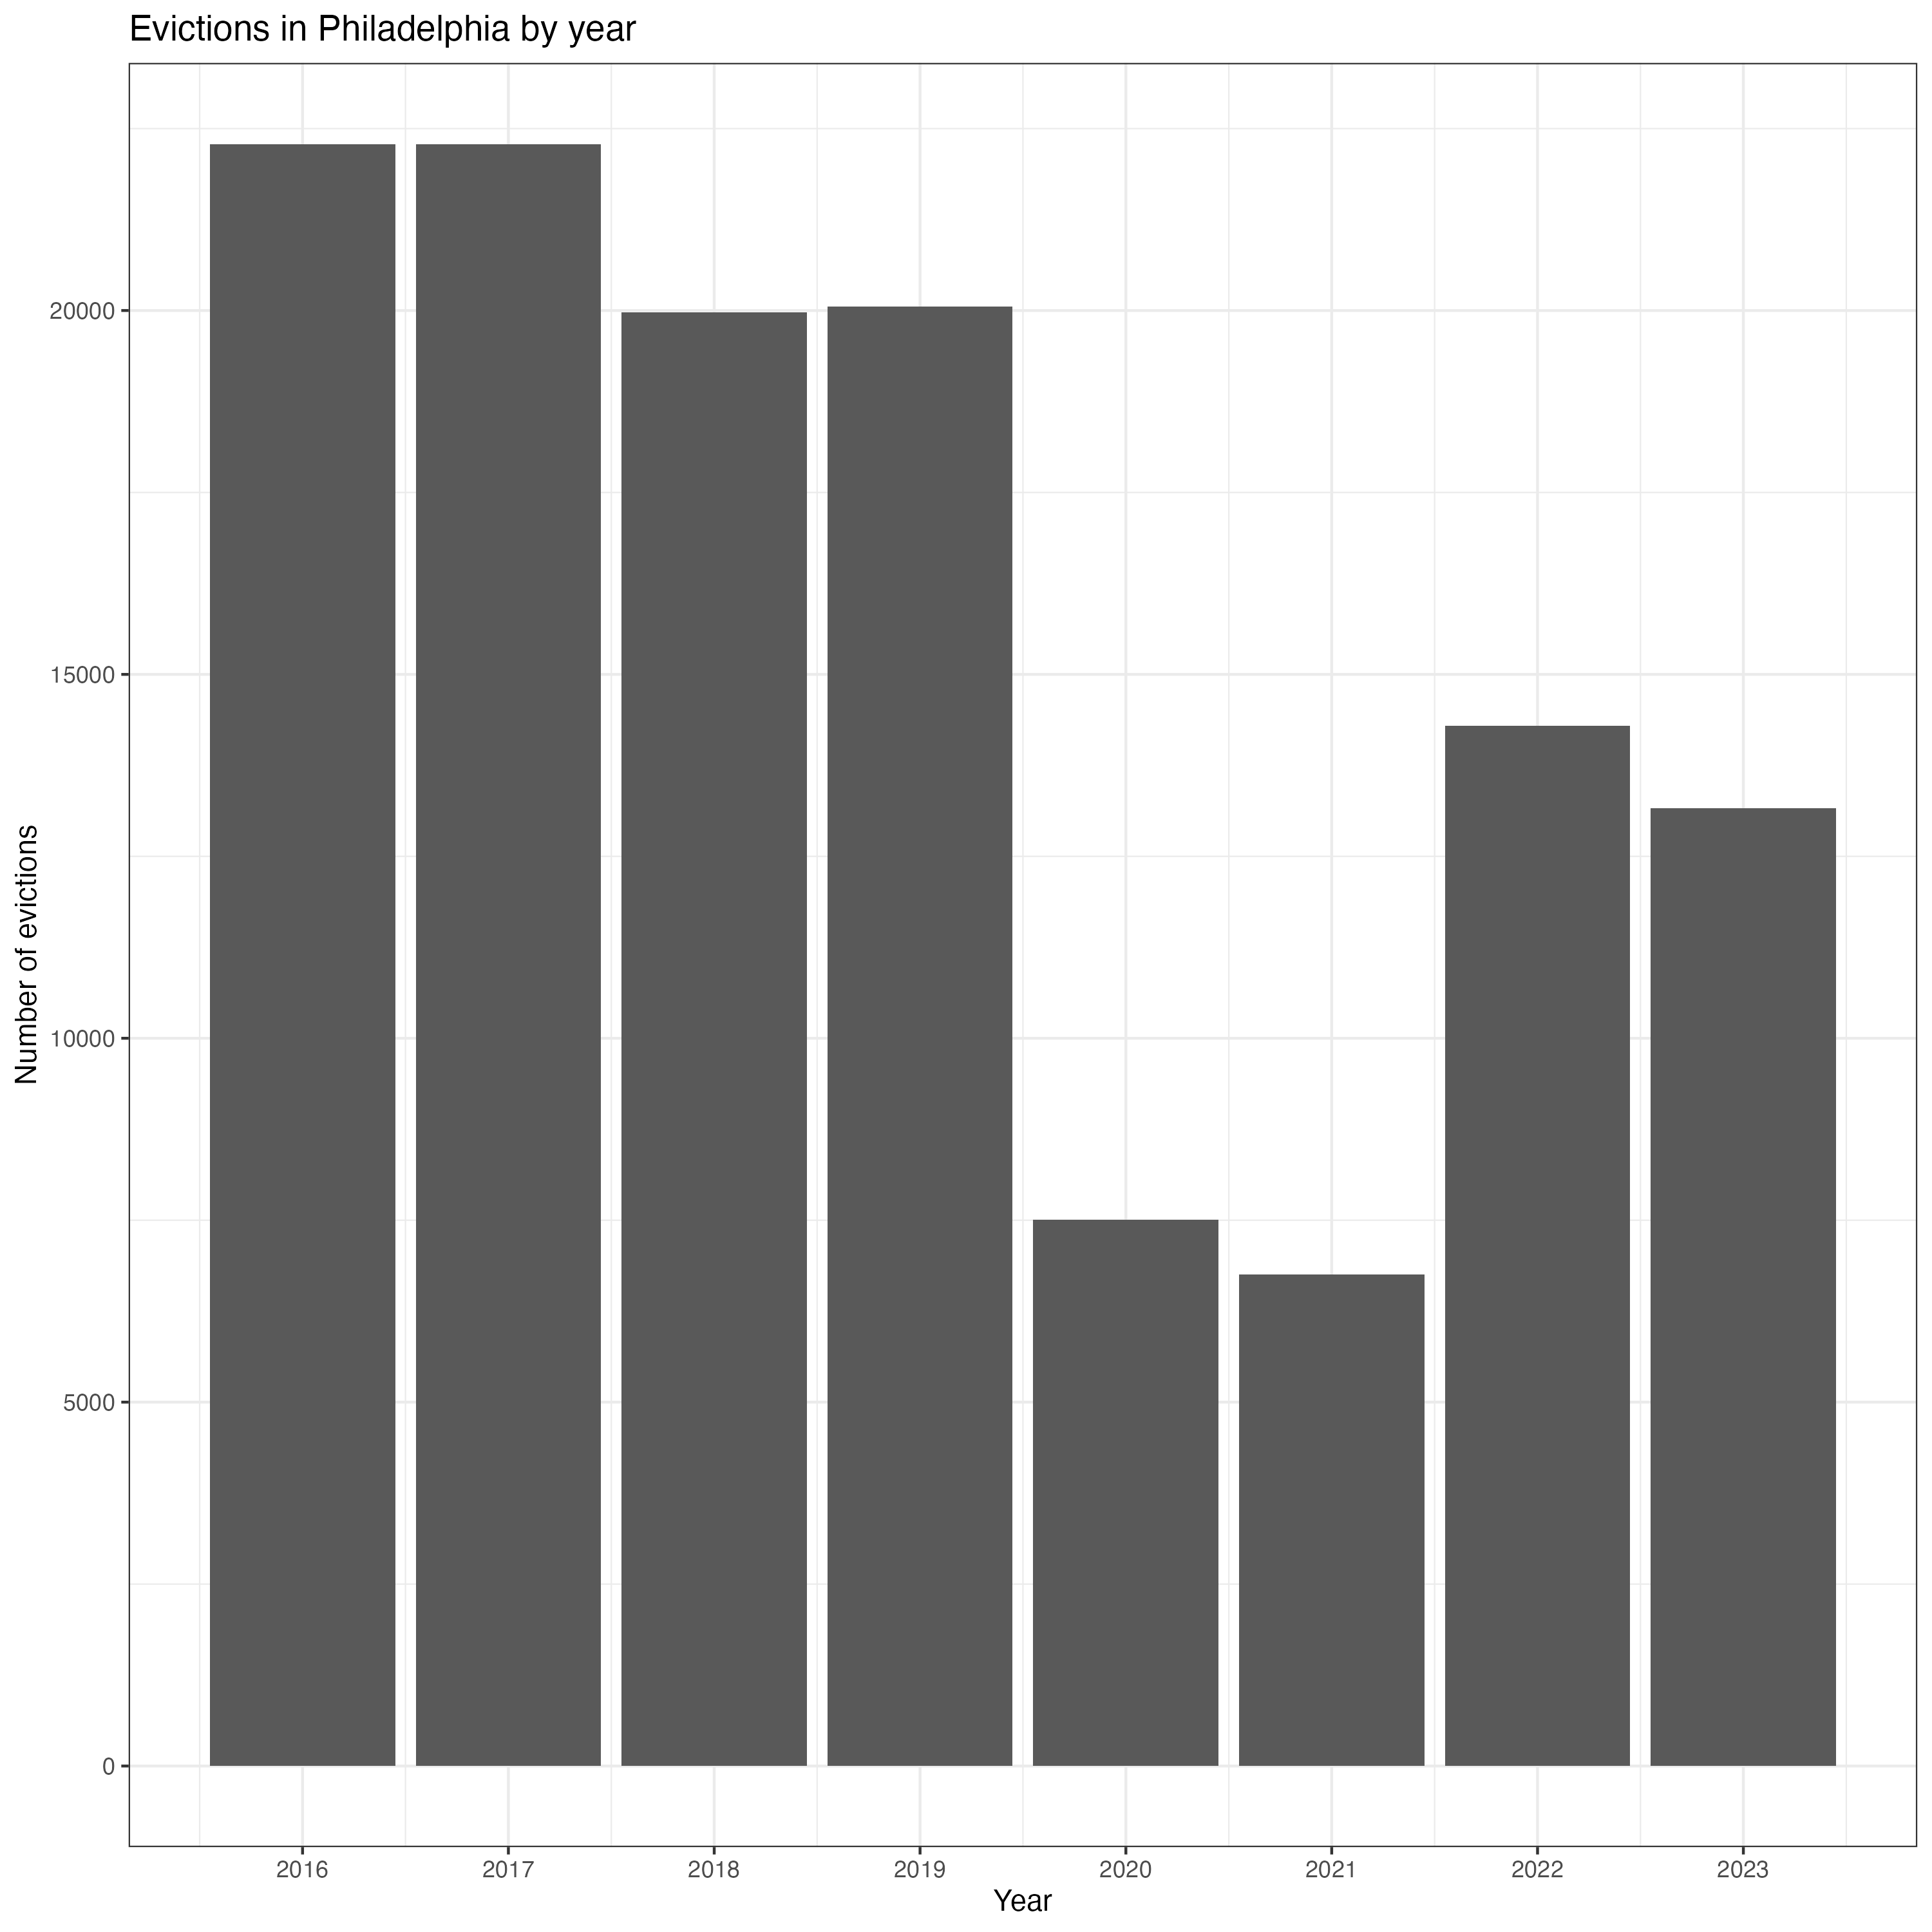
\includegraphics[width=1\linewidth]{figs/evict_by_year.png}
%     \caption{Evictions in Philadelphia}
%     \label{fig:philly-year}
% \end{figure}

% Taken together, these empirical facts show that there are interesting patterns of spatial clustering, patterns of landlord behavior, and possible policy variation I could exploit.
% \pagebreak
% \section{Research Questions and Empirical Specifications}

% \subsection{Descriptive Evidence on Pricing and Eviction Filing Behavior}

% The first set of findings I'd like to document are related to landlord pricing and filing behavior. Specifically:

% \begin{itemize}
%     \item Do high evicting landlords charge higher rents relative to similar properties?
%     \item Are thresholds (back rent required for eviction filing to occur) for high evicting landlords different from those for lower evicting landlords. 
%     \item Building on Alison Lodermeier's job market paper, a natural question would be whether high evicting landlords are more likely to statistically or tasted-basely discriminate against their tenants, relative to lower evicting landlords 
%     \item Are high evicting landlords also likely to be serial evictors -- meaning they use eviction both as a debt collection tool and as one to remove tenants.
% \end{itemize} \\

% As these are all descriptive findings, I think the identification is relatively straightforward. The main consideration will be what "similar property" means -- I think for now it will be defined geographically, assuming there aren't large rental gradients within the same neighborhood.



\end{document}